\documentclass[a4paper,11pt]{article}

% encoding UTF-8
\usepackage{ucs}
\usepackage[utf8x]{inputenc}

\usepackage[USenglish]{babel}
\usepackage{graphicx}
\usepackage{pslatex} % nicer times font

\newcommand{\myauthor}{Alejandro R. Mosteo}
\newcommand{\mytitle}{Virtual Network Specification}

\usepackage[        % Hyperlinks, PDF metadata
    unicode=true,
    pdfauthor={\myauthor},
    pdftitle ={\mytitle}
]{hyperref}         % It's best to load this last, it seems
\usepackage{hypcap} % fix references to captions to point to the figure proper
                    % This is the only package that should go after hyperref

\begin{document}

\author{\myauthor}
\title{\mytitle}
\maketitle

\section{Introduction \& scope.}

This document defines terminology used in the design and implementation of the virtual network component in the ACTION and ROSACE projects. It also describes the relationships among processes running during simulation, real missions and mixed experiments. This network is 'virtual' because it provides to agents a unified view of the transport layer, which can be internally be implemented by a number of different means, ranging from entirely simulated models to different real bridged networks using sophisticated routing protocols. 

By using this virtual network, the following objectives are achieved:

\begin{itemize}
    \item Communicating agents are isolated from any particularities of the underlying network, by means of a well-defined API that captures all agent needs (and, conversely, all network services). This API is thus the boundary between agent and network code.
    \item Different network instances can be used transparently:
        \begin{itemize}
            \item Simulation of different propagation models (perfect communication, distance-limited, line-of-sight based, etc.)
            \item Deployment of different real network layers: Wi-Fi, GSM, etc.
            \item Complex networking environments making use of any combination of the previous examples.
        \end{itemize}
    \item Monitoring of communications is simplified because all entry and exit points are homogeneous.
    \item \dots
\end{itemize}


\section{Definitions.}

Some terms that have a precise meaning in the descriptions that will follow are defined here. These definitions will be further expanded within their respective contexts.

\begin{description}
    \newcommand{\define}[2]{\item[#1:]\hfill\\#2.}
    
    \define{Agent}{An entity making use of the network services; e.g. real or simulated robots, planning stations, or other networked devices}
    
    \define{API}{Application Programming Interface; in this particular case, the services made available by the virtual network to agents}
    
    \define{vNet}{Virtual network being deployed. This comprises all processes that simulate or implement the actual data transport layer, from message sending to delivery. This virtual network provides all necessary networking facilities to agents in the context of the ACTION and ROSACE projects}
    
    \define{vProxy}{An entity locally available to every agent, which provides the API necessary to make use of the vNet. All interactions between an agent and the vNet are done through a vProxy. The vProxy is local to the agent in the sense that this link can be always established and should never fail (e.g. processes running in the same machine, or in different machines connected by reliable means. In particular, the first version of the vNet will use YARP for the interaction agent-vProxy, and thus permits that agent and vProxy are not in the same machine, as long as they are under the same YARP nameserver}
    
    %\define{vHub}{An entity that participates somehow in the internal implementation of the network, contributing to routing}
    
\end{description}

\section{Roadmap \& use cases.}

In this section, several use cases for the vNet are described, in increasing order of complexity, that should clarify the roles of each entity.

\subsection{Centralized simulation.}

The simplest case happens when robots are simulated and they are using a network model that does not require any inputs from the simulated world (e.g. perfect communication, fixed drop rate, etc):

\begin{center}
\includegraphics[width=0.666\columnwidth]{figures/central}
\end{center}

Each robot sends and receives messages via a single vProxy (formerly known as vHub). This vProxy centralizes and performs the network simulation. In the case of perfect communication, only routing is needed; with fixed drop rates, a simple random test is performed, and so on.

In the slightly more complex case of a network model that requires knowledge on the endpoints state (e.g. distance or line-of-sight), the schema would be, when using the MORSE simulator:

\begin{center}
\includegraphics[width=0.666\columnwidth]{figures/central+morse}
\end{center}

In this case, the vProxy queries the MORSE instance in order to determine if the messages can be delivered.

\subsection{Experiment with guaranteed communication backbone}

In the case of ACTION, there is a monitoring network that guarantees communications among agents. This network is not intended for direct agent use, but to guarantee full monitoring and control of the experiment. The vNet then simulates any lossy network model during experiments. The existence of this network, however, makes possible the use of the same setup as in a centralized simulation, if desired. This simplifies the logging and synchronization implementation (which can happen at a central place).

\subsection{Decentralized vNet simulation}

As a preparatory step for totally distributed execution in ROSACE, the following schema could be used:

\begin{center}
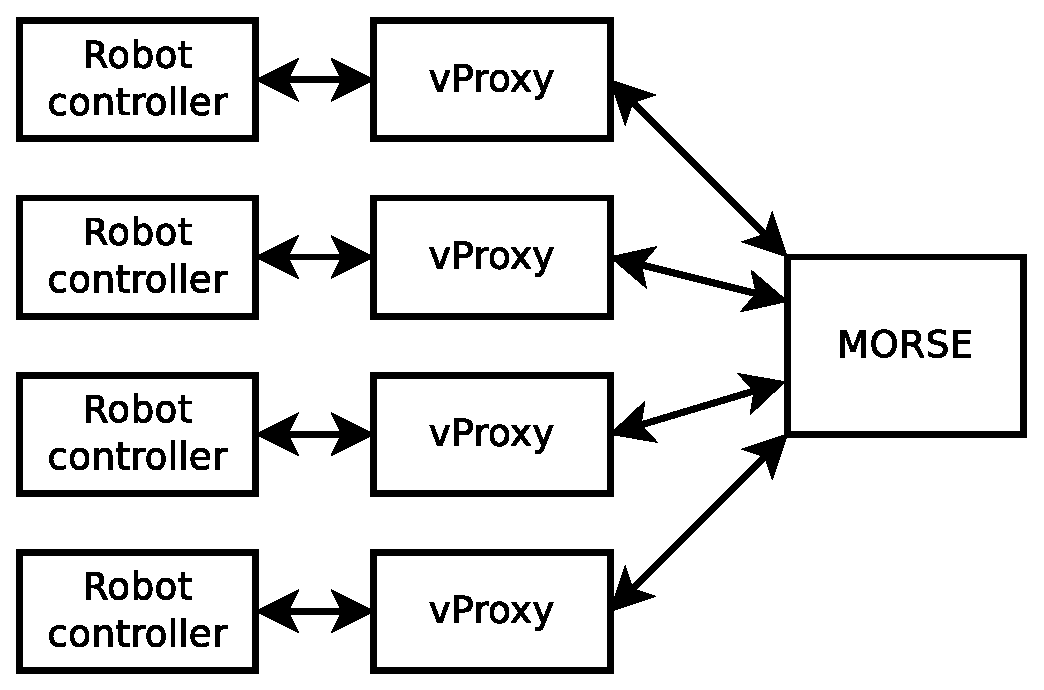
\includegraphics[width=0.666\columnwidth]{figures/distrib+morse}
\end{center}

Note that MORSE instances can be one (currently) or many (in the future). Since, in the case of multiple MORSE instances, it is expected that they all will have synchronized views of robots state, vProxies could connect to any available MORSE instance without need for changes.

\subsection{Distributed experiment without guaranteed communication}

In the more general case (and in ROSACE in particular), communication cannot be guaranteed among agents:

\begin{center}
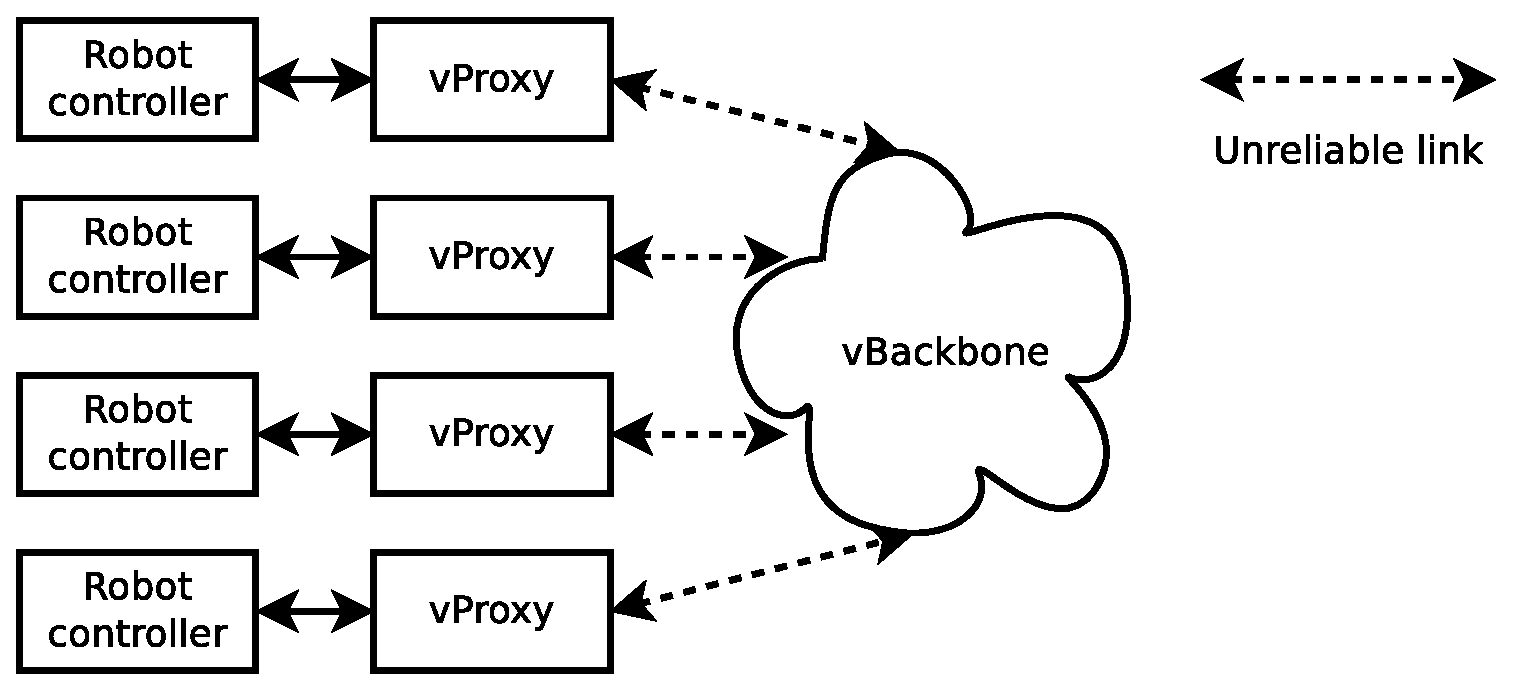
\includegraphics[width=0.666\columnwidth]{figures/distrib}
\end{center}

The cloud in the previous figure represents the actual network being used to communicate the agents. This network is provided by the communication services of work package ?.

\section{Class diagram for the general case.}

Here is an schema that depicts all envisioned entities and interactions, both visible to agents and invisible (implementation related). As a tentative design diagram, these entities are abstract classes whose particular instances could be defined in some configuration file, for example, or given via command-line parameters.

\begin{center}
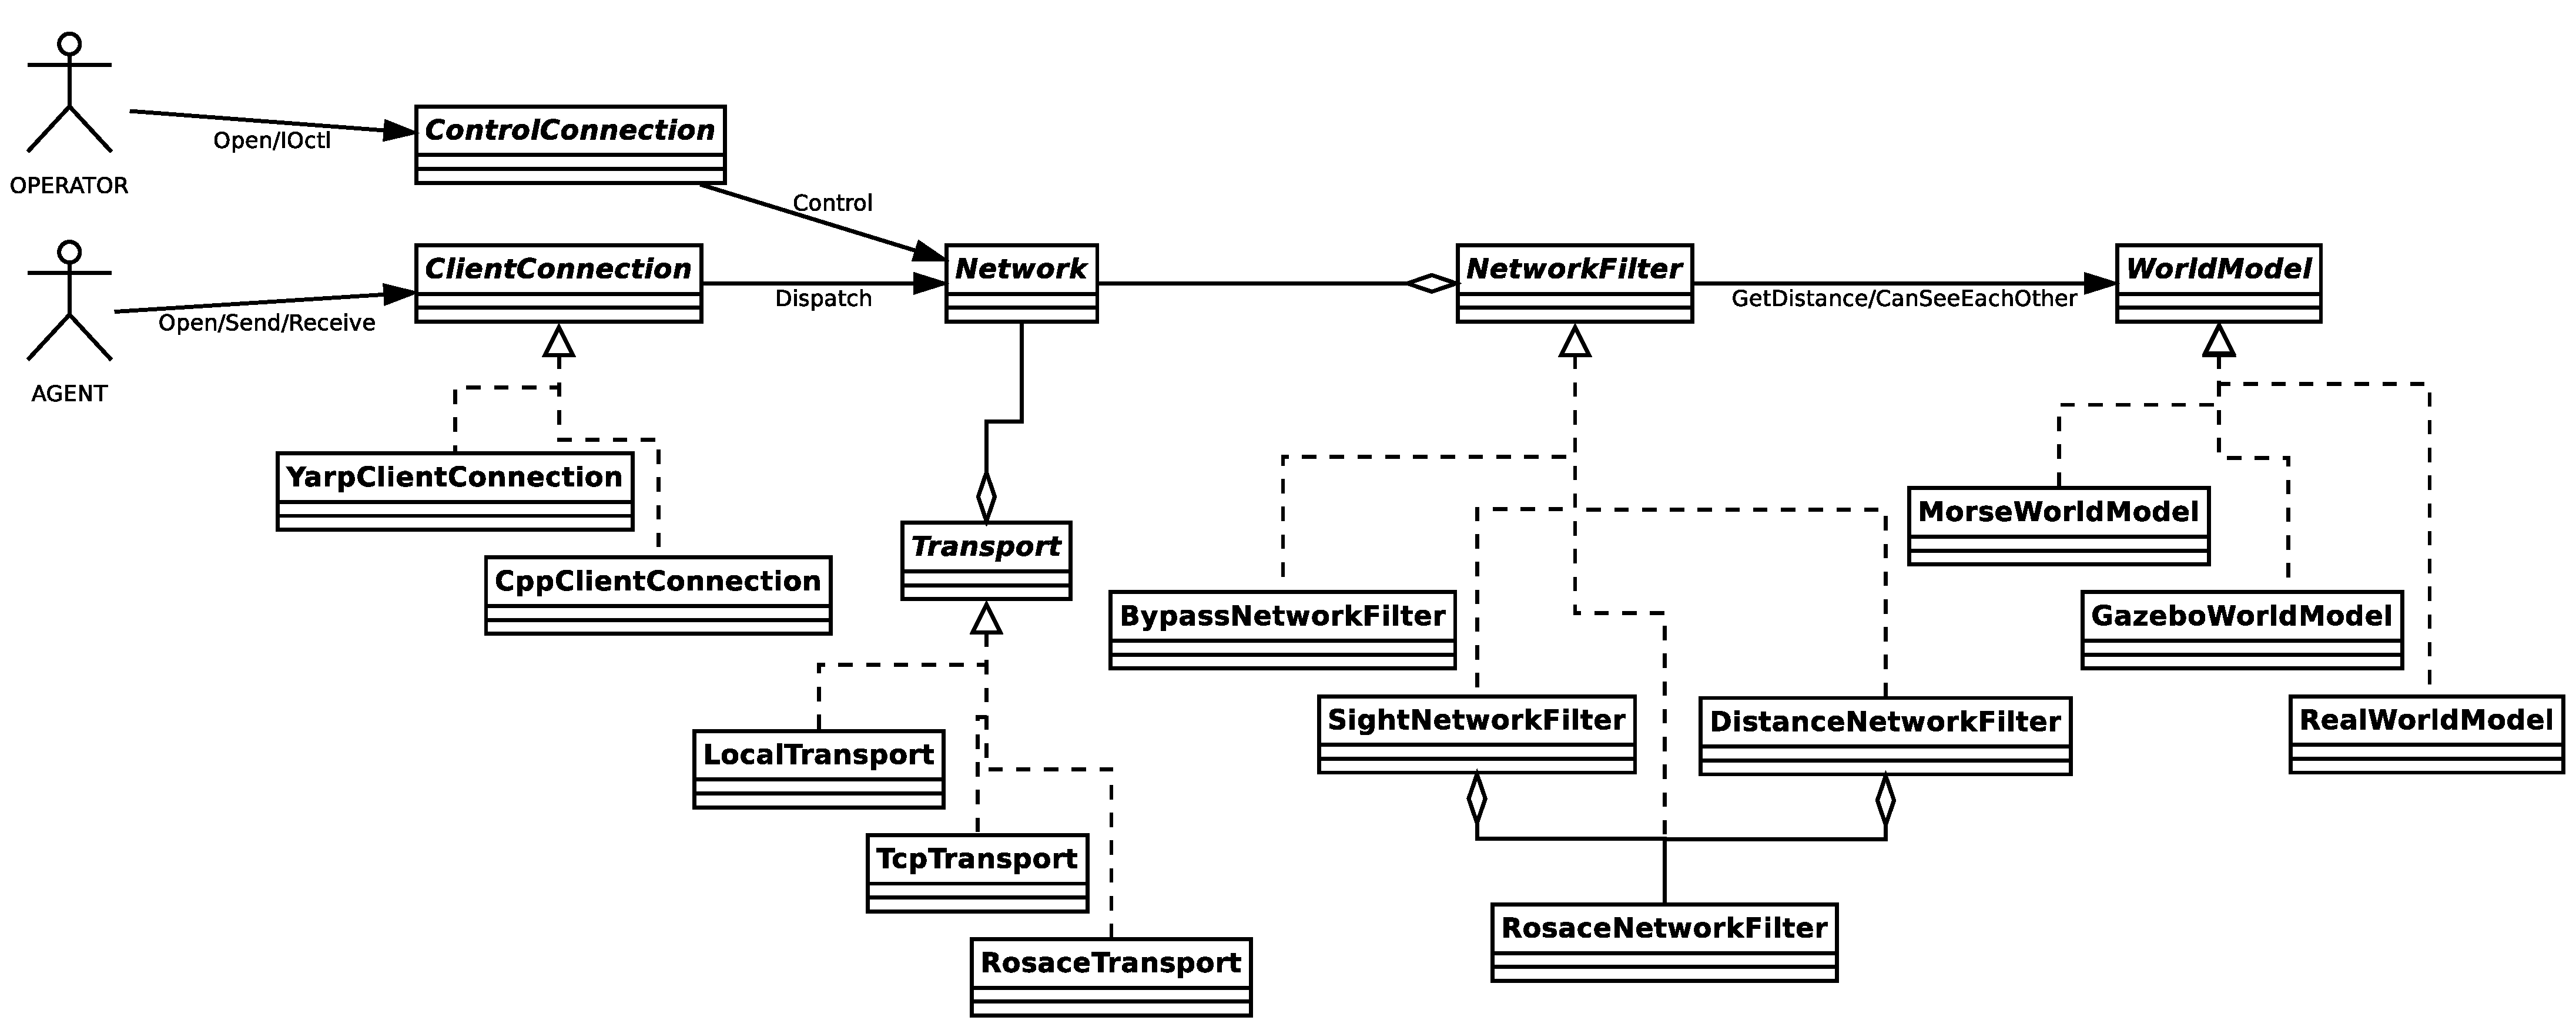
\includegraphics[width=0.999\columnwidth]{figures/classes}
\end{center}

\end{document}
